\documentclass[aspectratio=169,11pt]{beamer}
% =====================================================================
%  pds-beamer.tex — Estilo común de las transparencias.
%
%  Uso (desde teoría/Tx/transparencias/):
%     \documentclass[aspectratio=169,11pt]{beamer}
%     % =====================================================================
%  pds-beamer.tex — Estilo común de las transparencias.
%
%  Uso (desde teoría/Tx/transparencias/):
%     \documentclass[aspectratio=169,11pt]{beamer}
%     % =====================================================================
%  pds-beamer.tex — Estilo común de las transparencias.
%
%  Uso (desde teoría/Tx/transparencias/):
%     \documentclass[aspectratio=169,11pt]{beamer}
%     \input{../../comun/pds-beamer}
%     \title{...}  \subtitle{Tema x · ...}
%     \begin{document}
%       \portada
%       ...
%     \end{document}
%  Compilar con:  latexmk -xelatex  (o «make» desde teoría/)
% =====================================================================

\usetheme{Boadilla}
\usecolortheme{orchid}
\usefonttheme{professionalfonts}
\setbeamercovered{transparent}
\setbeamersize{text margin left=0.8cm, text margin right=0.8cm}
\setbeamertemplate{navigation symbols}{}
\setbeamertemplate{itemize item}[square]
\setbeamertemplate{itemize subitem}[circle]
\setbeamertemplate{itemize subsubitem}[triangle]
\setbeamertemplate{enumerate item}[square]
\setbeamertemplate{enumerate subitem}[circle]
\setbeamertemplate{caption}{\raggedright\insertcaption\par}

\input{../../comun/pds-comun.tex}

% Tipografía: Fira Sans + Fira Math (legibles en proyector)
\usepackage{fontspec}
\usepackage{unicode-math}
% Se cargan por nombre de fichero para que funcionen con cualquier
% instalación de TeX Live (o MiKTeX) sin instalar fuentes en el sistema.
\setmainfont{FiraSans}[Extension=.otf, UprightFont=*-Regular, BoldFont=*-SemiBold,
  ItalicFont=*-Italic, BoldItalicFont=*-SemiBoldItalic]
\setsansfont{FiraSans}[Extension=.otf, UprightFont=*-Regular, BoldFont=*-SemiBold,
  ItalicFont=*-Italic, BoldItalicFont=*-SemiBoldItalic]
\setmonofont{FiraMono}[Extension=.otf, UprightFont=*-Regular, BoldFont=*-Medium, AutoFakeSlant=0.15, Scale=0.92]
\setmathfont{FiraMath-Regular.otf}
\setmathfont{latinmodern-math.otf}[range={"229B,"22EE,"22F1}]

% Colores del tema ajustados a la paleta común (más contraste)
\setbeamercolor{structure}{fg=pdsazul}
\setbeamercolor{alerted text}{fg=pdsrojo}
\setbeamercolor{example text}{fg=pdsverde}
\setbeamercolor{block title}{bg=pdsazul, fg=white}
\setbeamercolor{block body}{bg=pdsfondo}
\setbeamercolor{block title alerted}{bg=pdsrojo, fg=white}
\setbeamercolor{block body alerted}{bg=pdsrojo!6}
\setbeamercolor{block title example}{bg=pdsverde, fg=white}
\setbeamercolor{block body example}{bg=pdsverde!6}
\setbeamercolor{frametitle}{fg=pdsazul, bg=white}
\setbeamerfont{frametitle}{size=\large, series=\bfseries}
\setbeamerfont{block title}{size=\normalsize, series=\bfseries}
\setbeamertemplate{blocks}[rounded][shadow=false]

% Logo en la esquina superior derecha de cada transparencia
\pgfdeclareimage[height=0.8cm]{logo}{../../comun/ucm.png}
\addtobeamertemplate{frametitle}{}{%
  \begin{tikzpicture}[remember picture, overlay]
    \node[anchor=north east, inner sep=0pt] at ([xshift=-0.25cm, yshift=-0.2cm]current page.north east) {\pgfuseimage{logo}};
  \end{tikzpicture}}

% Datos de portada
\author[\autorescorto]{\autores}
\institute[UCM]{\footnotesize\departamento\\\universidad}
\date[\curso]{\footnotesize\grado\\\curso}

\newcommand{\portada}{%
  \begin{frame}[plain]
    \begin{center}
      
\includegraphics[height=1.9cm]{../../comun/ucm.png}
    \end{center}
    \vspace{-0.4cm}
    \titlepage
  \end{frame}}

% Índice al empezar cada sección
\AtBeginSection[]{%
  \begin{frame}{Contenido}
    \tableofcontents[currentsection, hideothersubsections]
  \end{frame}}

\renewcommand{\pdscodesize}{\scriptsize}

% Utilidades
% \herramienta{T1-convolucion-continua}: enlace a la página publicada de
% herramientas/html (se abre en el navegador, sin instalar nada).
% \herramientaservidor{server/....py}: app que necesita Python (bokeh serve).
\newcommand{\urlherramientas}{https://ucm-237.github.io/PdS/}
\newcommand{\herramienta}[1]{%
  \par\vfill\hfill{\scriptsize\color{pdsgris}\faIcon\ \href{\urlherramientas#1.html}{Herramienta interactiva: \texttt{#1}}}}
\newcommand{\herramientaservidor}[1]{%
  \par\vfill\hfill{\scriptsize\color{pdsgris}\faIcon\ Herramienta interactiva (con Python): \texttt{herramientas/#1}}}
\newcommand{\faIcon}{\textbf{▶}}
\newcommand{\gris}[1]{{\color{pdsgris}#1}}
\newcommand{\nota}[1]{\par\vspace{2pt}{\footnotesize\color{pdsgris}\textit{#1}}\par}
% Nota sobre una errata de versiones anteriores (solo con \ERRATAS)
\newcommand{\errata}[1]{\iferratas\nota{Errata de versiones anteriores: #1}\fi}
\newcommand{\apuntes}[1]{\nota{Más detalle en los apuntes, #1.}}

% Bloques con nombre en castellano
\newenvironment{definicion}[1][Definición]{\begin{block}{#1}}{\end{block}}
\newenvironment{importante}[1][Importante]{\begin{alertblock}{#1}}{\end{alertblock}}
\newenvironment{ejemplo}[1][Ejemplo]{\begin{exampleblock}{#1}}{\end{exampleblock}}

%     \title{...}  \subtitle{Tema x · ...}
%     \begin{document}
%       \portada
%       ...
%     \end{document}
%  Compilar con:  latexmk -xelatex  (o «make» desde teoría/)
% =====================================================================

\usetheme{Boadilla}
\usecolortheme{orchid}
\usefonttheme{professionalfonts}
\setbeamercovered{transparent}
\setbeamersize{text margin left=0.8cm, text margin right=0.8cm}
\setbeamertemplate{navigation symbols}{}
\setbeamertemplate{itemize item}[square]
\setbeamertemplate{itemize subitem}[circle]
\setbeamertemplate{itemize subsubitem}[triangle]
\setbeamertemplate{enumerate item}[square]
\setbeamertemplate{enumerate subitem}[circle]
\setbeamertemplate{caption}{\raggedright\insertcaption\par}

% =====================================================================
%  pds-comun.tex — Paquetes, colores y estilos de código comunes a
%  transparencias, apuntes y hojas de ejercicios. Compilar con XeLaTeX.
%  No cargar directamente: lo cargan pds-beamer.tex y pds-apuntes.tex.
% =====================================================================

\usepackage{polyglossia}
\setmainlanguage{spanish}
\usepackage{mathtools}
\usepackage{graphicx}
\usepackage{booktabs}
\usepackage{multirow}
\usepackage{array}
\usepackage{xcolor}
\usepackage{tikz}
\usetikzlibrary{positioning,arrows.meta,calc,shapes.geometric,decorations.pathreplacing}
\usepackage{listings}
\usepackage{siunitx}
\sisetup{output-decimal-marker={,}, group-separator={\,}, per-mode=symbol}

% Notas de erratas de versiones anteriores: no se imprimen salvo que se
% defina \ERRATAS antes de cargar el estilo (make ERRATAS=1)
\newif\iferratas
\ifdefined\ERRATAS \erratastrue \fi

% Ruta común (logo y figuras compartidas)
\providecommand{\rutacomun}{../../comun/}
\input{\rutacomun datos.tex}

% ---------------------------------------------------------------------
%  Paleta (la misma que usan las figuras generadas con Python,
%  ver comun/pds_estilo.py)
% ---------------------------------------------------------------------
\definecolor{pdsazul}{HTML}{2B3A8C}
\definecolor{pdsrojo}{HTML}{C0392B}
\definecolor{pdsverde}{HTML}{1E7B4F}
\definecolor{pdsnaranja}{HTML}{D9822B}
\definecolor{pdsgris}{HTML}{5A5A66}
\definecolor{pdsfondo}{HTML}{F3F4FA}
\definecolor{pdscodigo}{HTML}{F7F7F2}

% ---------------------------------------------------------------------
%  Diagramas de bloques (TikZ)
% ---------------------------------------------------------------------
\tikzset{
  bloque/.style={rectangle, rounded corners=2pt, draw=pdsazul!80, fill=pdsfondo,
                 very thick, minimum height=8mm, minimum width=14mm, align=center},
  sumador/.style={circle, draw=pdsazul!80, fill=pdsfondo, thick, inner sep=1.5pt},
  flecha/.style={-{Stealth[length=2.2mm]}, thick, pdsgris},
}

% ---------------------------------------------------------------------
%  Código: Python y Matlab en paralelo
% ---------------------------------------------------------------------
\newcommand{\pdscodesize}{\footnotesize}
\lstdefinestyle{pds}{
  basicstyle=\ttfamily\pdscodesize,
  keywordstyle=\color{pdsazul}\bfseries,
  commentstyle=\color{pdsverde}\itshape,
  stringstyle=\color{pdsrojo},
  numbers=none,
  backgroundcolor=\color{pdscodigo},
  frame=single, rulecolor=\color{pdsgris!40}, framerule=0.4pt,
  xleftmargin=2pt, xrightmargin=2pt, aboveskip=2pt, belowskip=2pt,
  columns=fullflexible, keepspaces=true,
  showstringspaces=false, breaklines=true, tabsize=4,
  upquote=true,
  % Con XeLaTeX, listings desordena los caracteres no ASCII junto a
  % dígitos («2π» sale «π2»): se sustituyen por su versión matemática.
  literate={π}{{$\pi$}}1 {δ}{{$\delta$}}1 {ω}{{$\omega$}}1 {Ω}{{$\Omega$}}1
           {≈}{{$\approx$}}1 {µ}{{$\mu$}}1 {·}{{$\cdot$}}1 {α}{{$\alpha$}}1
           {á}{{á}}1 {é}{{é}}1 {í}{{í}}1 {ó}{{ó}}1 {ú}{{ú}}1 {ñ}{{ñ}}1 {¿}{{¿}}1,
}
\lstdefinestyle{python}{style=pds, language=Python,
  morekeywords={as,True,False,None}}
\lstdefinestyle{matlab}{style=pds, language=Matlab,
  morekeywords={function,end,true,false}}

% \codigo{<ruta sin extensión>} muestra el mismo ejemplo en Python
% y en Matlab, uno al lado del otro. Los ficheros viven en
% ../codigo/python/<nombre>.py y ../codigo/matlab/<nombre>.m y se
% ejecutan en las pruebas (make prueba-codigo).
\newcommand{\rutacodigo}{../codigo/}
\newcommand{\codigoetiqueta}[1]{{\sffamily\scriptsize\bfseries\color{pdsgris}#1}}
\newcommand{\codigo}[2][]{%
  \par\noindent
  \begin{minipage}[t]{0.495\linewidth}
    \codigoetiqueta{Python}\par\vspace{1pt}
    \lstinputlisting[style=python,#1]{\rutacodigo python/#2.py}
  \end{minipage}\hfill
  \begin{minipage}[t]{0.495\linewidth}
    \codigoetiqueta{Matlab}\par\vspace{1pt}
    \lstinputlisting[style=matlab,#1]{\rutacodigo matlab/#2.m}
  \end{minipage}\par}

\input{\rutacomun notacion.tex}


% Tipografía: Fira Sans + Fira Math (legibles en proyector)
\usepackage{fontspec}
\usepackage{unicode-math}
% Se cargan por nombre de fichero para que funcionen con cualquier
% instalación de TeX Live (o MiKTeX) sin instalar fuentes en el sistema.
\setmainfont{FiraSans}[Extension=.otf, UprightFont=*-Regular, BoldFont=*-SemiBold,
  ItalicFont=*-Italic, BoldItalicFont=*-SemiBoldItalic]
\setsansfont{FiraSans}[Extension=.otf, UprightFont=*-Regular, BoldFont=*-SemiBold,
  ItalicFont=*-Italic, BoldItalicFont=*-SemiBoldItalic]
\setmonofont{FiraMono}[Extension=.otf, UprightFont=*-Regular, BoldFont=*-Medium, AutoFakeSlant=0.15, Scale=0.92]
\setmathfont{FiraMath-Regular.otf}
\setmathfont{latinmodern-math.otf}[range={"229B,"22EE,"22F1}]

% Colores del tema ajustados a la paleta común (más contraste)
\setbeamercolor{structure}{fg=pdsazul}
\setbeamercolor{alerted text}{fg=pdsrojo}
\setbeamercolor{example text}{fg=pdsverde}
\setbeamercolor{block title}{bg=pdsazul, fg=white}
\setbeamercolor{block body}{bg=pdsfondo}
\setbeamercolor{block title alerted}{bg=pdsrojo, fg=white}
\setbeamercolor{block body alerted}{bg=pdsrojo!6}
\setbeamercolor{block title example}{bg=pdsverde, fg=white}
\setbeamercolor{block body example}{bg=pdsverde!6}
\setbeamercolor{frametitle}{fg=pdsazul, bg=white}
\setbeamerfont{frametitle}{size=\large, series=\bfseries}
\setbeamerfont{block title}{size=\normalsize, series=\bfseries}
\setbeamertemplate{blocks}[rounded][shadow=false]

% Logo en la esquina superior derecha de cada transparencia
\pgfdeclareimage[height=0.8cm]{logo}{../../comun/ucm.png}
\addtobeamertemplate{frametitle}{}{%
  \begin{tikzpicture}[remember picture, overlay]
    \node[anchor=north east, inner sep=0pt] at ([xshift=-0.25cm, yshift=-0.2cm]current page.north east) {\pgfuseimage{logo}};
  \end{tikzpicture}}

% Datos de portada
\author[\autorescorto]{\autores}
\institute[UCM]{\footnotesize\departamento\\\universidad}
\date[\curso]{\footnotesize\grado\\\curso}

\newcommand{\portada}{%
  \begin{frame}[plain]
    \begin{center}
      
\includegraphics[height=1.9cm]{../../comun/ucm.png}
    \end{center}
    \vspace{-0.4cm}
    \titlepage
  \end{frame}}

% Índice al empezar cada sección
\AtBeginSection[]{%
  \begin{frame}{Contenido}
    \tableofcontents[currentsection, hideothersubsections]
  \end{frame}}

\renewcommand{\pdscodesize}{\scriptsize}

% Utilidades
% \herramienta{T1-convolucion-continua}: enlace a la página publicada de
% herramientas/html (se abre en el navegador, sin instalar nada).
% \herramientaservidor{server/....py}: app que necesita Python (bokeh serve).
\newcommand{\urlherramientas}{https://ucm-237.github.io/PdS/}
\newcommand{\herramienta}[1]{%
  \par\vfill\hfill{\scriptsize\color{pdsgris}\faIcon\ \href{\urlherramientas#1.html}{Herramienta interactiva: \texttt{#1}}}}
\newcommand{\herramientaservidor}[1]{%
  \par\vfill\hfill{\scriptsize\color{pdsgris}\faIcon\ Herramienta interactiva (con Python): \texttt{herramientas/#1}}}
\newcommand{\faIcon}{\textbf{▶}}
\newcommand{\gris}[1]{{\color{pdsgris}#1}}
\newcommand{\nota}[1]{\par\vspace{2pt}{\footnotesize\color{pdsgris}\textit{#1}}\par}
% Nota sobre una errata de versiones anteriores (solo con \ERRATAS)
\newcommand{\errata}[1]{\iferratas\nota{Errata de versiones anteriores: #1}\fi}
\newcommand{\apuntes}[1]{\nota{Más detalle en los apuntes, #1.}}

% Bloques con nombre en castellano
\newenvironment{definicion}[1][Definición]{\begin{block}{#1}}{\end{block}}
\newenvironment{importante}[1][Importante]{\begin{alertblock}{#1}}{\end{alertblock}}
\newenvironment{ejemplo}[1][Ejemplo]{\begin{exampleblock}{#1}}{\end{exampleblock}}

%     \title{...}  \subtitle{Tema x · ...}
%     \begin{document}
%       \portada
%       ...
%     \end{document}
%  Compilar con:  latexmk -xelatex  (o «make» desde teoría/)
% =====================================================================

\usetheme{Boadilla}
\usecolortheme{orchid}
\usefonttheme{professionalfonts}
\setbeamercovered{transparent}
\setbeamersize{text margin left=0.8cm, text margin right=0.8cm}
\setbeamertemplate{navigation symbols}{}
\setbeamertemplate{itemize item}[square]
\setbeamertemplate{itemize subitem}[circle]
\setbeamertemplate{itemize subsubitem}[triangle]
\setbeamertemplate{enumerate item}[square]
\setbeamertemplate{enumerate subitem}[circle]
\setbeamertemplate{caption}{\raggedright\insertcaption\par}

% =====================================================================
%  pds-comun.tex — Paquetes, colores y estilos de código comunes a
%  transparencias, apuntes y hojas de ejercicios. Compilar con XeLaTeX.
%  No cargar directamente: lo cargan pds-beamer.tex y pds-apuntes.tex.
% =====================================================================

\usepackage{polyglossia}
\setmainlanguage{spanish}
\usepackage{mathtools}
\usepackage{graphicx}
\usepackage{booktabs}
\usepackage{multirow}
\usepackage{array}
\usepackage{xcolor}
\usepackage{tikz}
\usetikzlibrary{positioning,arrows.meta,calc,shapes.geometric,decorations.pathreplacing}
\usepackage{listings}
\usepackage{siunitx}
\sisetup{output-decimal-marker={,}, group-separator={\,}, per-mode=symbol}

% Notas de erratas de versiones anteriores: no se imprimen salvo que se
% defina \ERRATAS antes de cargar el estilo (make ERRATAS=1)
\newif\iferratas
\ifdefined\ERRATAS \erratastrue \fi

% Ruta común (logo y figuras compartidas)
\providecommand{\rutacomun}{../../comun/}
\input{\rutacomun datos.tex}

% ---------------------------------------------------------------------
%  Paleta (la misma que usan las figuras generadas con Python,
%  ver comun/pds_estilo.py)
% ---------------------------------------------------------------------
\definecolor{pdsazul}{HTML}{2B3A8C}
\definecolor{pdsrojo}{HTML}{C0392B}
\definecolor{pdsverde}{HTML}{1E7B4F}
\definecolor{pdsnaranja}{HTML}{D9822B}
\definecolor{pdsgris}{HTML}{5A5A66}
\definecolor{pdsfondo}{HTML}{F3F4FA}
\definecolor{pdscodigo}{HTML}{F7F7F2}

% ---------------------------------------------------------------------
%  Diagramas de bloques (TikZ)
% ---------------------------------------------------------------------
\tikzset{
  bloque/.style={rectangle, rounded corners=2pt, draw=pdsazul!80, fill=pdsfondo,
                 very thick, minimum height=8mm, minimum width=14mm, align=center},
  sumador/.style={circle, draw=pdsazul!80, fill=pdsfondo, thick, inner sep=1.5pt},
  flecha/.style={-{Stealth[length=2.2mm]}, thick, pdsgris},
}

% ---------------------------------------------------------------------
%  Código: Python y Matlab en paralelo
% ---------------------------------------------------------------------
\newcommand{\pdscodesize}{\footnotesize}
\lstdefinestyle{pds}{
  basicstyle=\ttfamily\pdscodesize,
  keywordstyle=\color{pdsazul}\bfseries,
  commentstyle=\color{pdsverde}\itshape,
  stringstyle=\color{pdsrojo},
  numbers=none,
  backgroundcolor=\color{pdscodigo},
  frame=single, rulecolor=\color{pdsgris!40}, framerule=0.4pt,
  xleftmargin=2pt, xrightmargin=2pt, aboveskip=2pt, belowskip=2pt,
  columns=fullflexible, keepspaces=true,
  showstringspaces=false, breaklines=true, tabsize=4,
  upquote=true,
  % Con XeLaTeX, listings desordena los caracteres no ASCII junto a
  % dígitos («2π» sale «π2»): se sustituyen por su versión matemática.
  literate={π}{{$\pi$}}1 {δ}{{$\delta$}}1 {ω}{{$\omega$}}1 {Ω}{{$\Omega$}}1
           {≈}{{$\approx$}}1 {µ}{{$\mu$}}1 {·}{{$\cdot$}}1 {α}{{$\alpha$}}1
           {á}{{á}}1 {é}{{é}}1 {í}{{í}}1 {ó}{{ó}}1 {ú}{{ú}}1 {ñ}{{ñ}}1 {¿}{{¿}}1,
}
\lstdefinestyle{python}{style=pds, language=Python,
  morekeywords={as,True,False,None}}
\lstdefinestyle{matlab}{style=pds, language=Matlab,
  morekeywords={function,end,true,false}}

% \codigo{<ruta sin extensión>} muestra el mismo ejemplo en Python
% y en Matlab, uno al lado del otro. Los ficheros viven en
% ../codigo/python/<nombre>.py y ../codigo/matlab/<nombre>.m y se
% ejecutan en las pruebas (make prueba-codigo).
\newcommand{\rutacodigo}{../codigo/}
\newcommand{\codigoetiqueta}[1]{{\sffamily\scriptsize\bfseries\color{pdsgris}#1}}
\newcommand{\codigo}[2][]{%
  \par\noindent
  \begin{minipage}[t]{0.495\linewidth}
    \codigoetiqueta{Python}\par\vspace{1pt}
    \lstinputlisting[style=python,#1]{\rutacodigo python/#2.py}
  \end{minipage}\hfill
  \begin{minipage}[t]{0.495\linewidth}
    \codigoetiqueta{Matlab}\par\vspace{1pt}
    \lstinputlisting[style=matlab,#1]{\rutacodigo matlab/#2.m}
  \end{minipage}\par}

\input{\rutacomun notacion.tex}


% Tipografía: Fira Sans + Fira Math (legibles en proyector)
\usepackage{fontspec}
\usepackage{unicode-math}
% Se cargan por nombre de fichero para que funcionen con cualquier
% instalación de TeX Live (o MiKTeX) sin instalar fuentes en el sistema.
\setmainfont{FiraSans}[Extension=.otf, UprightFont=*-Regular, BoldFont=*-SemiBold,
  ItalicFont=*-Italic, BoldItalicFont=*-SemiBoldItalic]
\setsansfont{FiraSans}[Extension=.otf, UprightFont=*-Regular, BoldFont=*-SemiBold,
  ItalicFont=*-Italic, BoldItalicFont=*-SemiBoldItalic]
\setmonofont{FiraMono}[Extension=.otf, UprightFont=*-Regular, BoldFont=*-Medium, AutoFakeSlant=0.15, Scale=0.92]
\setmathfont{FiraMath-Regular.otf}
\setmathfont{latinmodern-math.otf}[range={"229B,"22EE,"22F1}]

% Colores del tema ajustados a la paleta común (más contraste)
\setbeamercolor{structure}{fg=pdsazul}
\setbeamercolor{alerted text}{fg=pdsrojo}
\setbeamercolor{example text}{fg=pdsverde}
\setbeamercolor{block title}{bg=pdsazul, fg=white}
\setbeamercolor{block body}{bg=pdsfondo}
\setbeamercolor{block title alerted}{bg=pdsrojo, fg=white}
\setbeamercolor{block body alerted}{bg=pdsrojo!6}
\setbeamercolor{block title example}{bg=pdsverde, fg=white}
\setbeamercolor{block body example}{bg=pdsverde!6}
\setbeamercolor{frametitle}{fg=pdsazul, bg=white}
\setbeamerfont{frametitle}{size=\large, series=\bfseries}
\setbeamerfont{block title}{size=\normalsize, series=\bfseries}
\setbeamertemplate{blocks}[rounded][shadow=false]

% Logo en la esquina superior derecha de cada transparencia
\pgfdeclareimage[height=0.8cm]{logo}{../../comun/ucm.png}
\addtobeamertemplate{frametitle}{}{%
  \begin{tikzpicture}[remember picture, overlay]
    \node[anchor=north east, inner sep=0pt] at ([xshift=-0.25cm, yshift=-0.2cm]current page.north east) {\pgfuseimage{logo}};
  \end{tikzpicture}}

% Datos de portada
\author[\autorescorto]{\autores}
\institute[UCM]{\footnotesize\departamento\\\universidad}
\date[\curso]{\footnotesize\grado\\\curso}

\newcommand{\portada}{%
  \begin{frame}[plain]
    \begin{center}
      
\includegraphics[height=1.9cm]{../../comun/ucm.png}
    \end{center}
    \vspace{-0.4cm}
    \titlepage
  \end{frame}}

% Índice al empezar cada sección
\AtBeginSection[]{%
  \begin{frame}{Contenido}
    \tableofcontents[currentsection, hideothersubsections]
  \end{frame}}

\renewcommand{\pdscodesize}{\scriptsize}

% Utilidades
% \herramienta{T1-convolucion-continua}: enlace a la página publicada de
% herramientas/html (se abre en el navegador, sin instalar nada).
% \herramientaservidor{server/....py}: app que necesita Python (bokeh serve).
\newcommand{\urlherramientas}{https://ucm-237.github.io/PdS/}
\newcommand{\herramienta}[1]{%
  \par\vfill\hfill{\scriptsize\color{pdsgris}\faIcon\ \href{\urlherramientas#1.html}{Herramienta interactiva: \texttt{#1}}}}
\newcommand{\herramientaservidor}[1]{%
  \par\vfill\hfill{\scriptsize\color{pdsgris}\faIcon\ Herramienta interactiva (con Python): \texttt{herramientas/#1}}}
\newcommand{\faIcon}{\textbf{▶}}
\newcommand{\gris}[1]{{\color{pdsgris}#1}}
\newcommand{\nota}[1]{\par\vspace{2pt}{\footnotesize\color{pdsgris}\textit{#1}}\par}
% Nota sobre una errata de versiones anteriores (solo con \ERRATAS)
\newcommand{\errata}[1]{\iferratas\nota{Errata de versiones anteriores: #1}\fi}
\newcommand{\apuntes}[1]{\nota{Más detalle en los apuntes, #1.}}

% Bloques con nombre en castellano
\newenvironment{definicion}[1][Definición]{\begin{block}{#1}}{\end{block}}
\newenvironment{importante}[1][Importante]{\begin{alertblock}{#1}}{\end{alertblock}}
\newenvironment{ejemplo}[1][Ejemplo]{\begin{exampleblock}{#1}}{\end{exampleblock}}

\graphicspath{{../figuras/}}

\title[T3 · DFT]{Transformada discreta de Fourier}
\subtitle{Tema 3 · Parte 1: de la DTFT a la DFT}

\begin{document}
\portada

% =====================================================================
\begin{frame}{Objetivos del tema}
  \begin{columns}[T]
    \begin{column}{0.52\textwidth}
      Calcular espectros con un computador y usarlos para analizar y filtrar señales:
      \begin{itemize}
        \item La \alert{DFT} como muestreo de la DTFT de una secuencia finita.
        \item Sus propiedades y la \alert{convolución circular}.
        \item Análisis espectral: resolución, fuga y \alert{ventanas}; espectrograma.
        \item La \alert{FFT} y la convolución rápida.
      \end{itemize}
    \end{column}
    \begin{column}{0.44\textwidth}
      \begin{block}{Material del tema}
        \small
        \begin{enumerate}
          \item De la DTFT a la DFT
          \item Propiedades y convolución circular
          \item Análisis espectral con la DFT
          \item FFT y convolución rápida
        \end{enumerate}
        \smallskip
        Apuntes, hoja de ejercicios y ejemplos en Python y Matlab.
      \end{block}
    \end{column}
  \end{columns}
\end{frame}

% =====================================================================
\section{Por qué otra transformada}

\begin{frame}{Recordatorio: la DTFT}
  \begin{definicion}[Transformada de Fourier de tiempo discreto (DTFT)]
    \[
      \Xd=\sum_{n=-\infty}^{\infty}x[n]\,\e^{-j\Omega n},\qquad
      x[n]=\frac{1}{2\pi}\int_{0}^{2\pi}\Xd\,\e^{j\Omega n}\dd\Omega
    \]
  \end{definicion}
  \begin{itemize}
    \item $\Xd$ es una función \alert{continua} de $\Omega$ y \alert{periódica} de periodo $2\pi$ (Tema~2: es el muestreo en el tiempo).
    \item Para calcularla con un computador hay dos obstáculos:
    \begin{itemize}
      \item la suma tiene \alert{infinitos términos}: solo conocemos un número finito de muestras;
      \item el resultado es una función de \alert{variable continua}: solo podemos guardar un número finito de valores.
    \end{itemize}
    \item La DFT resuelve los dos: trabaja con $N$ muestras en el tiempo y da $N$ muestras en frecuencia.
  \end{itemize}
\end{frame}

\begin{frame}{Primer obstáculo: solo tenemos $N$ muestras}
  \begin{columns}[c]
    \begin{column}{0.5\textwidth}
      \small
      Observar $N$ muestras es multiplicar por una \alert{ventana}:
      \[
        x_N[n]=x[n]\,w[n],\qquad w[n]=\begin{cases}1&0\le n<N\\0&\text{en otro caso}\end{cases}
      \]
      \[
        W(\e^{j\Omega})=\sum_{n=0}^{N-1}\e^{-j\Omega n}=\e^{-j\Omega\frac{N-1}{2}}\,\frac{\sin(\Omega N/2)}{\sin(\Omega/2)}
      \]
      Producto en el tiempo, \alert{convolución periódica} en frecuencia:
      \[
        X_N(\e^{j\Omega})=\frac{1}{2\pi}\int_{0}^{2\pi}X(\e^{j\theta})\,W\big(\e^{j(\Omega-\theta)}\big)\dd\theta
      \]
    \end{column}
    \begin{column}{0.48\textwidth}
      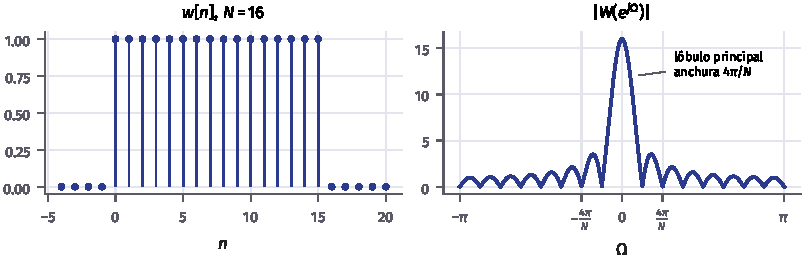
\includegraphics[width=\linewidth]{ventana_rect}
      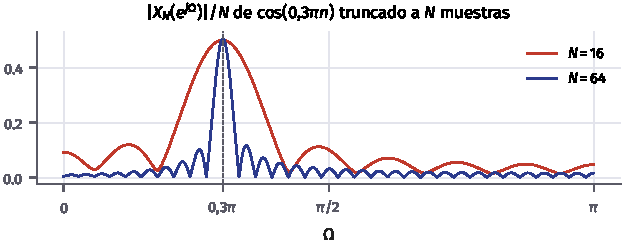
\includegraphics[width=\linewidth]{truncamiento}
    \end{column}
  \end{columns}
  \nota{Truncar la señal emborrona el espectro: cada línea se convierte en una copia de $W$. Cuanto mayor es $N$, más estrecho es el lóbulo principal (parte~3).}
\end{frame}

\begin{frame}{Segundo obstáculo: muestrear la DTFT}
  \begin{itemize}
    \item $N$ muestras equiespaciadas de un periodo, $\Omega\in[0,2\pi)$:
    \[
      \Omega_k=\frac{2\pi}{N}k,\qquad k=0,1,\dots,N-1,\qquad \text{separación }\Delta\Omega=\frac{2\pi}{N}.
    \]
    \item Si $x[n]$ solo es no nula en $0\le n<N$:
    \[
      X[k]=X(\e^{j\Omega})\big|_{\Omega=2\pi k/N}=\sum_{n=0}^{N-1}x[n]\,\e^{-j\frac{2\pi}{N}kn}
    \]
  \end{itemize}
  \begin{center}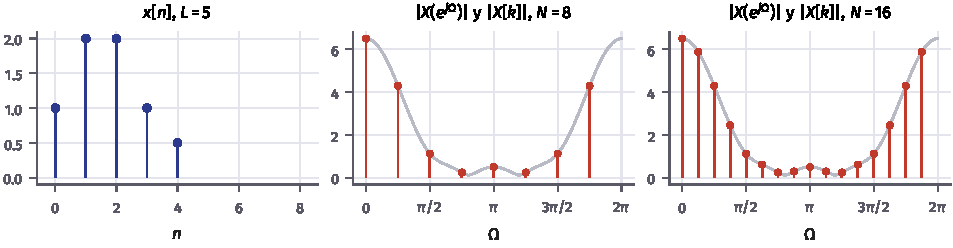
\includegraphics[height=0.26\textheight]{dtft_dft}\end{center}
  \nota{Con $N=16$ se ve mejor la forma de la DTFT, pero no hay más información: $x[n]$ es la misma.}
\end{frame}

% =====================================================================
\section{Definición}

\begin{frame}{La transformada discreta de Fourier}
  \begin{definicion}[DFT de $N$ puntos]
    \[
      X[k]=\sum_{n=0}^{N-1}x[n]\,W_N^{kn},\qquad
      x[n]=\frac{1}{N}\sum_{k=0}^{N-1}X[k]\,W_N^{-kn},\qquad
      W_N=\e^{-j2\pi/N}
    \]
    con $n,k=0,1,\dots,N-1$.
  \end{definicion}
  \begin{itemize}
    \item Transforma $N$ números (complejos) en $N$ números: es una transformación \alert{lineal e invertible}.
    \item La IDFT suma sobre $k$ y lleva el factor $1/N$; el signo del exponente es el contrario que en la DFT.
    \item $X[k]$ es la DTFT de la secuencia en $\Omega_k=2\pi k/N$: el índice $k$ es una frecuencia.
    \item $W_N$ es una raíz $N$-ésima de la unidad: $W_N^N=1$, $W_N^{N/2}=-1$, $W_N^{k+N}=W_N^k$.
  \end{itemize}
\end{frame}

\begin{frame}{Forma matricial}
  \begin{columns}[c]
    \begin{column}{0.56\textwidth}
      \small
      \[
        \begin{pmatrix}X[0]\\X[1]\\\vdots\\X[N-1]\end{pmatrix}=
        \begin{pmatrix}
          1&1&\cdots&1\\
          1&W_N&\cdots&W_N^{N-1}\\
          \vdots&\vdots&\ddots&\vdots\\
          1&W_N^{N-1}&\cdots&W_N^{(N-1)(N-1)}
        \end{pmatrix}
        \begin{pmatrix}x[0]\\x[1]\\\vdots\\x[N-1]\end{pmatrix}
      \]
      \[
        \mathbf X=\mathbf W_N\,\mathbf x,\qquad \mathbf x=\frac1N\,\mathbf W_N^{*}\,\mathbf X
      \]
      \begin{itemize}\small
        \item $\mathbf W_N$ es simétrica y $\mathbf W_N^{*}\mathbf W_N=N\mathbf I$: sus columnas son ortogonales.
        \item Cálculo directo: $N^2$ productos complejos. La FFT lo reduce a $\frac N2\log_2N$ (parte~4).
      \end{itemize}
    \end{column}
    \begin{column}{0.42\textwidth}
      \begin{ejemplo}[$N=4$, $x=(1,3,4,0)$]
        \footnotesize
        $W_4=\e^{-j\pi/2}=-j$:
        \[
          \mathbf W_4=\begin{pmatrix}1&1&1&1\\1&-j&-1&j\\1&-1&1&-1\\1&j&-1&-j\end{pmatrix}
        \]
        \[
          \mathbf X=(8,\ -3-3j,\ 2,\ -3+3j)
        \]
        $X[0]=\sum x[n]$ es la componente continua (8). $X[3]=X^*[1]$ porque $x$ es real.
      \end{ejemplo}
    \end{column}
  \end{columns}
\end{frame}

\begin{frame}{En código: la DFT como producto de matrices}
  \codigo{dft_directa}
  \nota{\texttt{fft} calcula exactamente lo mismo, pero en $O(N\log N)$ operaciones.}
\end{frame}

% =====================================================================
\section{Extensión periódica}

\begin{frame}{¿Qué secuencia recupera la IDFT?}
  Si $x[n]$ tiene cualquier longitud, agrupamos la DTFT muestreada en bloques de $N$ muestras:
  \[
    X[k]=\sum_{n=-\infty}^{\infty}x[n]\,W_N^{kn}=\sum_{n=0}^{N-1}\Big[\sum_{m=-\infty}^{\infty}x[n-mN]\Big]W_N^{kn},
  \]
  porque $W_N^{k(n-mN)}=W_N^{kn}$. La IDFT de las $N$ muestras devuelve un periodo de
  \begin{importante}[Extensión periódica]
    \vspace{-2mm}
    \[
      \tilde x[n]=\sum_{m=-\infty}^{\infty}x[n-mN]
    \]
    \vspace{-4mm}
  \end{importante}
  \begin{itemize}
    \item Muestrear en frecuencia \alert{periodiza} en el tiempo, igual que muestrear en el tiempo periodiza en frecuencia.
    \item $x[n]$ se recupera si tiene longitud finita $L$ y $N\ge L$. Si $N<L$, las copias se solapan: \alert{aliasing temporal}.
  \end{itemize}
\end{frame}

\begin{frame}{Aliasing en el tiempo}
  \begin{center}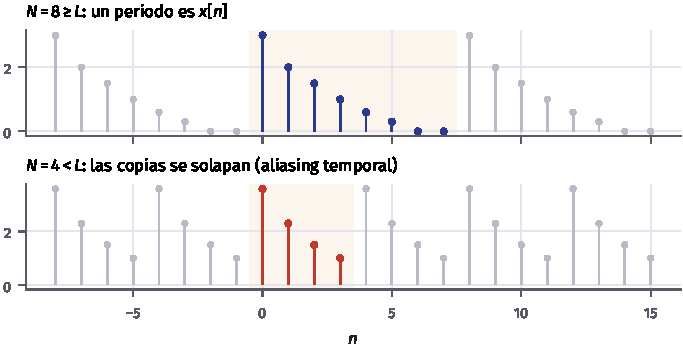
\includegraphics[height=0.45\textheight]{extension_periodica}\end{center}
  \begin{itemize}\small
    \item Con $N\ge L$ un periodo de $\tilde x[n]$ es exactamente $x[n]$ seguida de $N-L$ ceros.
    \item Con $N<L$ las muestras $n\ge N$ se suman a las del principio: $\tilde x[0]=x[0]+x[4]$, \dots
    \item Es el «teorema del muestreo en frecuencia»: $N$ muestras de la DTFT determinan una secuencia de longitud $L\le N$.
  \end{itemize}
  \herramienta{T3-extension-periodica}
\end{frame}

\begin{frame}{La DFT y la serie de Fourier discreta}
  \begin{itemize}
    \item Una secuencia periódica de periodo $N$ tiene serie de Fourier (Tema~1)
    \[
      \tilde x[n]=\sum_{k=0}^{N-1}c_k\,\e^{j\frac{2\pi}{N}kn},\qquad c_k=\frac1N\sum_{n=0}^{N-1}\tilde x[n]\,\e^{-j\frac{2\pi}{N}kn}
    \]
    \item Comparando con la DFT de un periodo: \alert{$X[k]=N\,c_k$}.
    \item La DFT trata la secuencia como si fuera \alert{un periodo de una señal periódica}. Por eso los índices se entienden siempre módulo $N$:
    \[
      x[n]\equiv x[((n))_N],\qquad X[k]\equiv X[((k))_N],\qquad ((n))_N=n\bmod N.
    \]
    \item Esta interpretación explica las propiedades «circulares» de la parte~2.
  \end{itemize}
\end{frame}

\begin{frame}{La DFT y la transformada Z}
  \begin{columns}[c]
    \begin{column}{0.55\textwidth}
      \begin{itemize}
        \item Como $\Xd=X(z)|_{z=\e^{j\Omega}}$:
        \[
          X[k]=X(z)\big|_{z=\e^{j2\pi k/N}}
        \]
        La DFT son $N$ muestras de $X(z)$ \alert{equiespaciadas en la circunferencia unidad}.
        \item Para una secuencia de longitud $\le N$, las $N$ muestras determinan $X(z)$ en todo el plano:
        \[
          X(z)=\frac{1-z^{-N}}{N}\sum_{k=0}^{N-1}\frac{X[k]}{1-W_N^{-k}z^{-1}}
        \]
      \end{itemize}
    \end{column}
    \begin{column}{0.42\textwidth}
      \begin{center}
        \begin{tikzpicture}[scale=1.5]
          \draw[->, pdsgris] (-1.3,0) -- (1.4,0) node[right, font=\footnotesize]{$\Re z$};
          \draw[->, pdsgris] (0,-1.3) -- (0,1.4) node[above, font=\footnotesize]{$\Im z$};
          \draw[pdsazul, thick] (0,0) circle (1);
          \foreach \k in {0,...,7} {
            \fill[pdsrojo] ({cos(45*\k)},{sin(45*\k)}) circle (1.6pt);
          }
          \node[font=\footnotesize, right] at (1,0.15) {$k=0$};
          \node[font=\footnotesize] at (0.95,0.95) {$k=1$};
          \node[font=\footnotesize, pdsgris] at (0,-1.55) {$N=8$};
        \end{tikzpicture}
      \end{center}
    \end{column}
  \end{columns}
\end{frame}

% =====================================================================
\section*{Resumen}
\begin{frame}{Conceptos importantes}
  \begin{columns}[T]
    \begin{column}{0.5\textwidth}
      \begin{itemize}
        \item Observar $N$ muestras es enventanar: el espectro se convoluciona con $W(\e^{j\Omega})$.
        \item DFT: $X[k]=\sum_{n=0}^{N-1}x[n]W_N^{kn}$, $W_N=\e^{-j2\pi/N}$.
        \item IDFT: $x[n]=\frac1N\sum_{k=0}^{N-1}X[k]W_N^{-kn}$.
        \item $X[k]$ es la DTFT en $\Omega_k=2\pi k/N$.
      \end{itemize}
    \end{column}
    \begin{column}{0.5\textwidth}
      \begin{itemize}
        \item Muestrear en frecuencia periodiza en el tiempo: la IDFT da $\tilde x[n]=\sum_mx[n-mN]$.
        \item Sin aliasing temporal si $N\ge L$.
        \item $X[k]=Nc_k$: la DFT ve un periodo de una señal periódica; índices módulo $N$.
        \item $X[k]$ son muestras de $X(z)$ en la circunferencia unidad.
      \end{itemize}
    \end{column}
  \end{columns}
  \bigskip
  \gris{Apuntes del Tema 3, secciones 1 y 2 · Hoja de ejercicios, ejercicios 1–4.}
  \herramienta{T3-dft}
\end{frame}

\end{document}
